\documentclass[a4paper,12pt]{article}
\usepackage{fullpage}
\usepackage[british]{babel}
\usepackage[T1]{fontenc}
\usepackage{amsmath}
\usepackage{amssymb}
\usepackage[T1]{fontenc}
\usepackage[latin1]{inputenc} 
\usepackage{amsthm} \newtheorem{theorem}{Theorem}
\usepackage{color}
\usepackage{float}

\usepackage{alltt}
\usepackage{listings}
 \usepackage{aeguill} 
\usepackage{dsfont}
%\usepackage{algorithm}
\usepackage[noend]{algorithm2e}
%\usepackage{algorithmicx}
\usepackage{subfig}
\lstset{% parameters for all code listings
	language=Python,
	frame=single,
	basicstyle=\small,  % nothing smaller than \footnotesize, please
	tabsize=2,
	numbers=left,
	framexleftmargin=2em,  % extend frame to include line numbers
	%xrightmargin=2em,  % extra space to fit 79 characters
	breaklines=true,
	breakatwhitespace=true,
	prebreak={/},
	captionpos=b,
	columns=fullflexible,
	escapeinside={\#*}{\^^M}
}


\usepackage{fancyvrb}
\DefineVerbatimEnvironment{code}{Verbatim}{fontsize=\small}
\DefineVerbatimEnvironment{example}{Verbatim}{fontsize=\small}

\usepackage{tikz} \usetikzlibrary{trees}
\usepackage{hyperref}  % should always be the last package

% useful colours (use sparingly!):
\newcommand{\blue}[1]{{\color{blue}#1}}
\newcommand{\green}[1]{{\color{green}#1}}
\newcommand{\red}[1]{{\color{red}#1}}

% useful wrappers for algorithmic/Python notation:
\newcommand{\length}[1]{\text{len}(#1)}
\newcommand{\twodots}{\mathinner{\ldotp\ldotp}}  % taken from clrscode3e.sty
\newcommand{\Oh}[1]{\mathcal{O}\left(#1\right)}

% useful (wrappers for) math symbols:
\newcommand{\Cardinality}[1]{\left\lvert#1\right\rvert}
%\newcommand{\Cardinality}[1]{\##1}
\newcommand{\Ceiling}[1]{\left\lceil#1\right\rceil}
\newcommand{\Floor}[1]{\left\lfloor#1\right\rfloor}
\newcommand{\Iff}{\Leftrightarrow}
\newcommand{\Implies}{\Rightarrow}
\newcommand{\Intersect}{\cap}
\newcommand{\Sequence}[1]{\left[#1\right]}
\newcommand{\Set}[1]{\left\{#1\right\}}
\newcommand{\SetComp}[2]{\Set{#1\SuchThat#2}}
\newcommand{\SuchThat}{\mid}
\newcommand{\Tuple}[1]{\langle#1\rangle}
\newcommand{\Union}{\cup}
\usetikzlibrary{positioning,shapes,shadows,arrows}


\title{\textbf{Separation of Voronoi Areas}}

\author{Martin Gebert, Sascha Schreckenbach, Jonathan Sharyari}  % replace by your name(s)

%\date{Month Day, Year}
\date{\today}

\begin{document}

\maketitle

\begin{figure}
\section*{\large Abstract}
....
\end{figure}
\newpage

\section{Introduction}
\subsection{Voronoi Diagram}
Given a set of points in space, a Voronoi diagram is a partitioning of the space into a set of Voronoi regions or "cells". The Voronoi region corresponding to a point \emph{p} consists of all points that are closer to \emph{p} than to any other point in space.

\begin{figure}[hb]
\centering
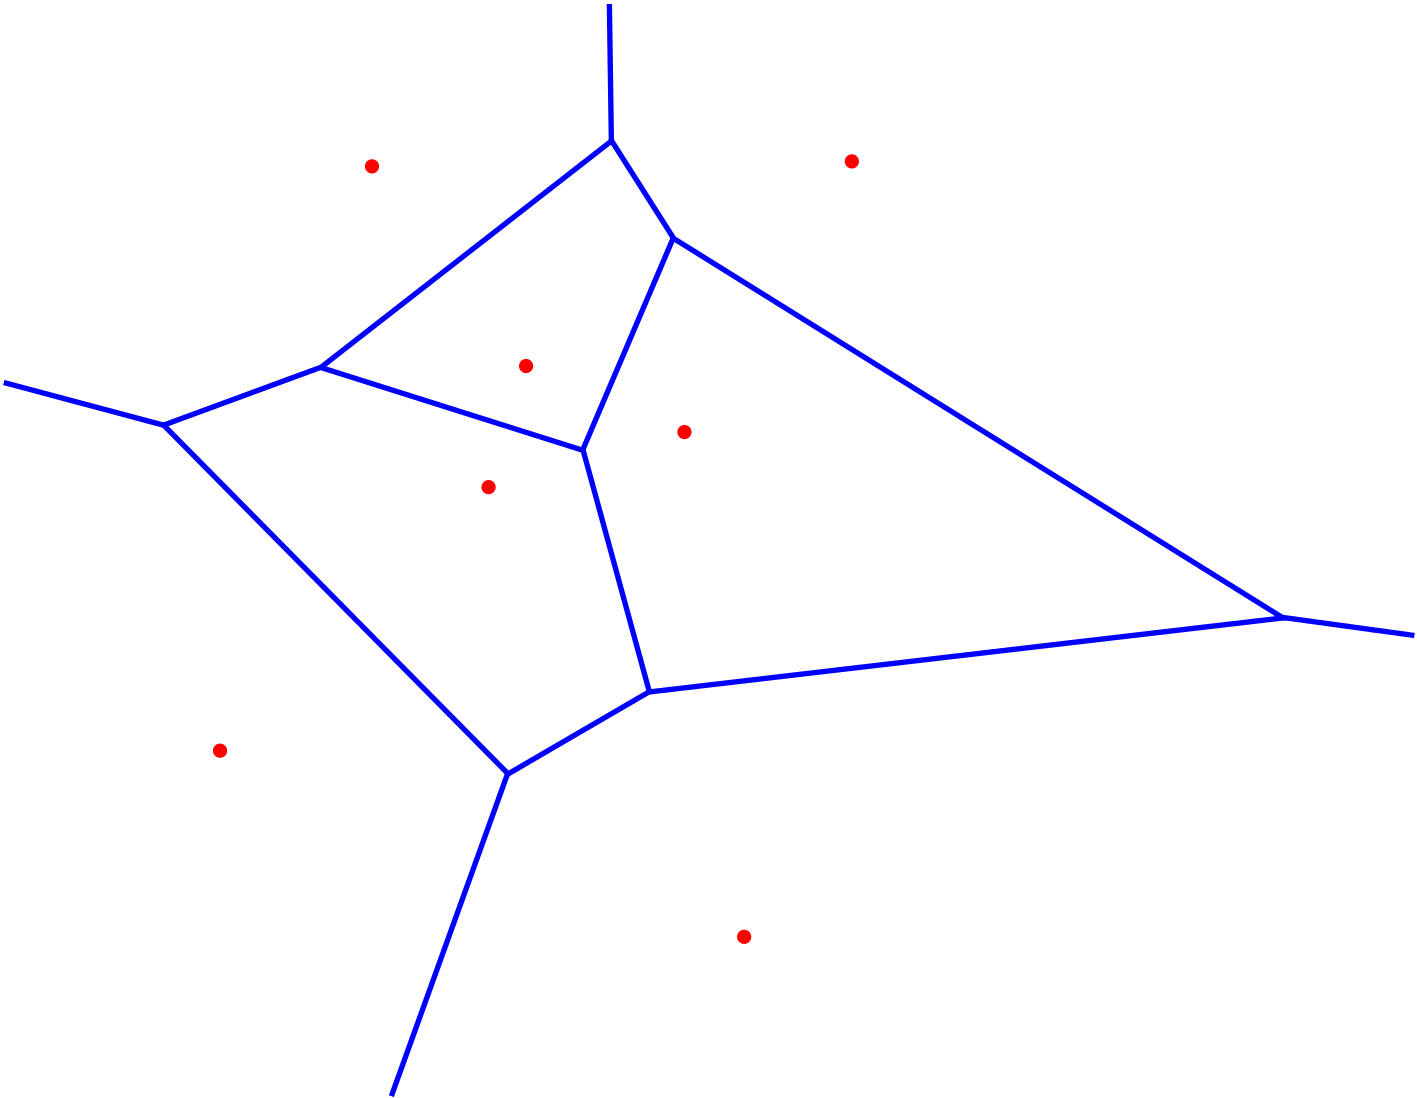
\includegraphics[width=0.4\textwidth]{pictures/Voronoi-diagram.png}
 \caption[Close up of \textit{Hemidactylus} sp.]
{A Voronoi diagram.}
\end{figure}

\subsection{Delaunay triangulation}
A Delaunay triangulation for a set of points in space is a triangulation of the points, with the added property that no point is inside the circumcircle of any triangle in the triangulation. \newline
The Delaunay triangulation is dual to the Voronoi diagram. 

\begin{figure}[hb]
\centering
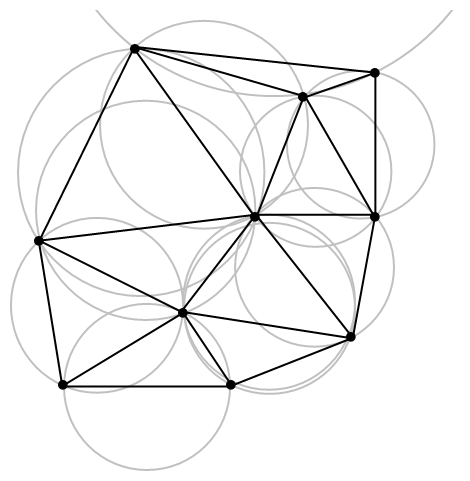
\includegraphics[width=0.4\textwidth]{pictures/Delaunay_circumcircles.png}
 \caption[Close up of \textit{Hemidactylus} sp.]
{A Delaunay triangulation, with a set of corresponding Delaunay circles.}
\end{figure}



\begin{figure}[hb]
\centering
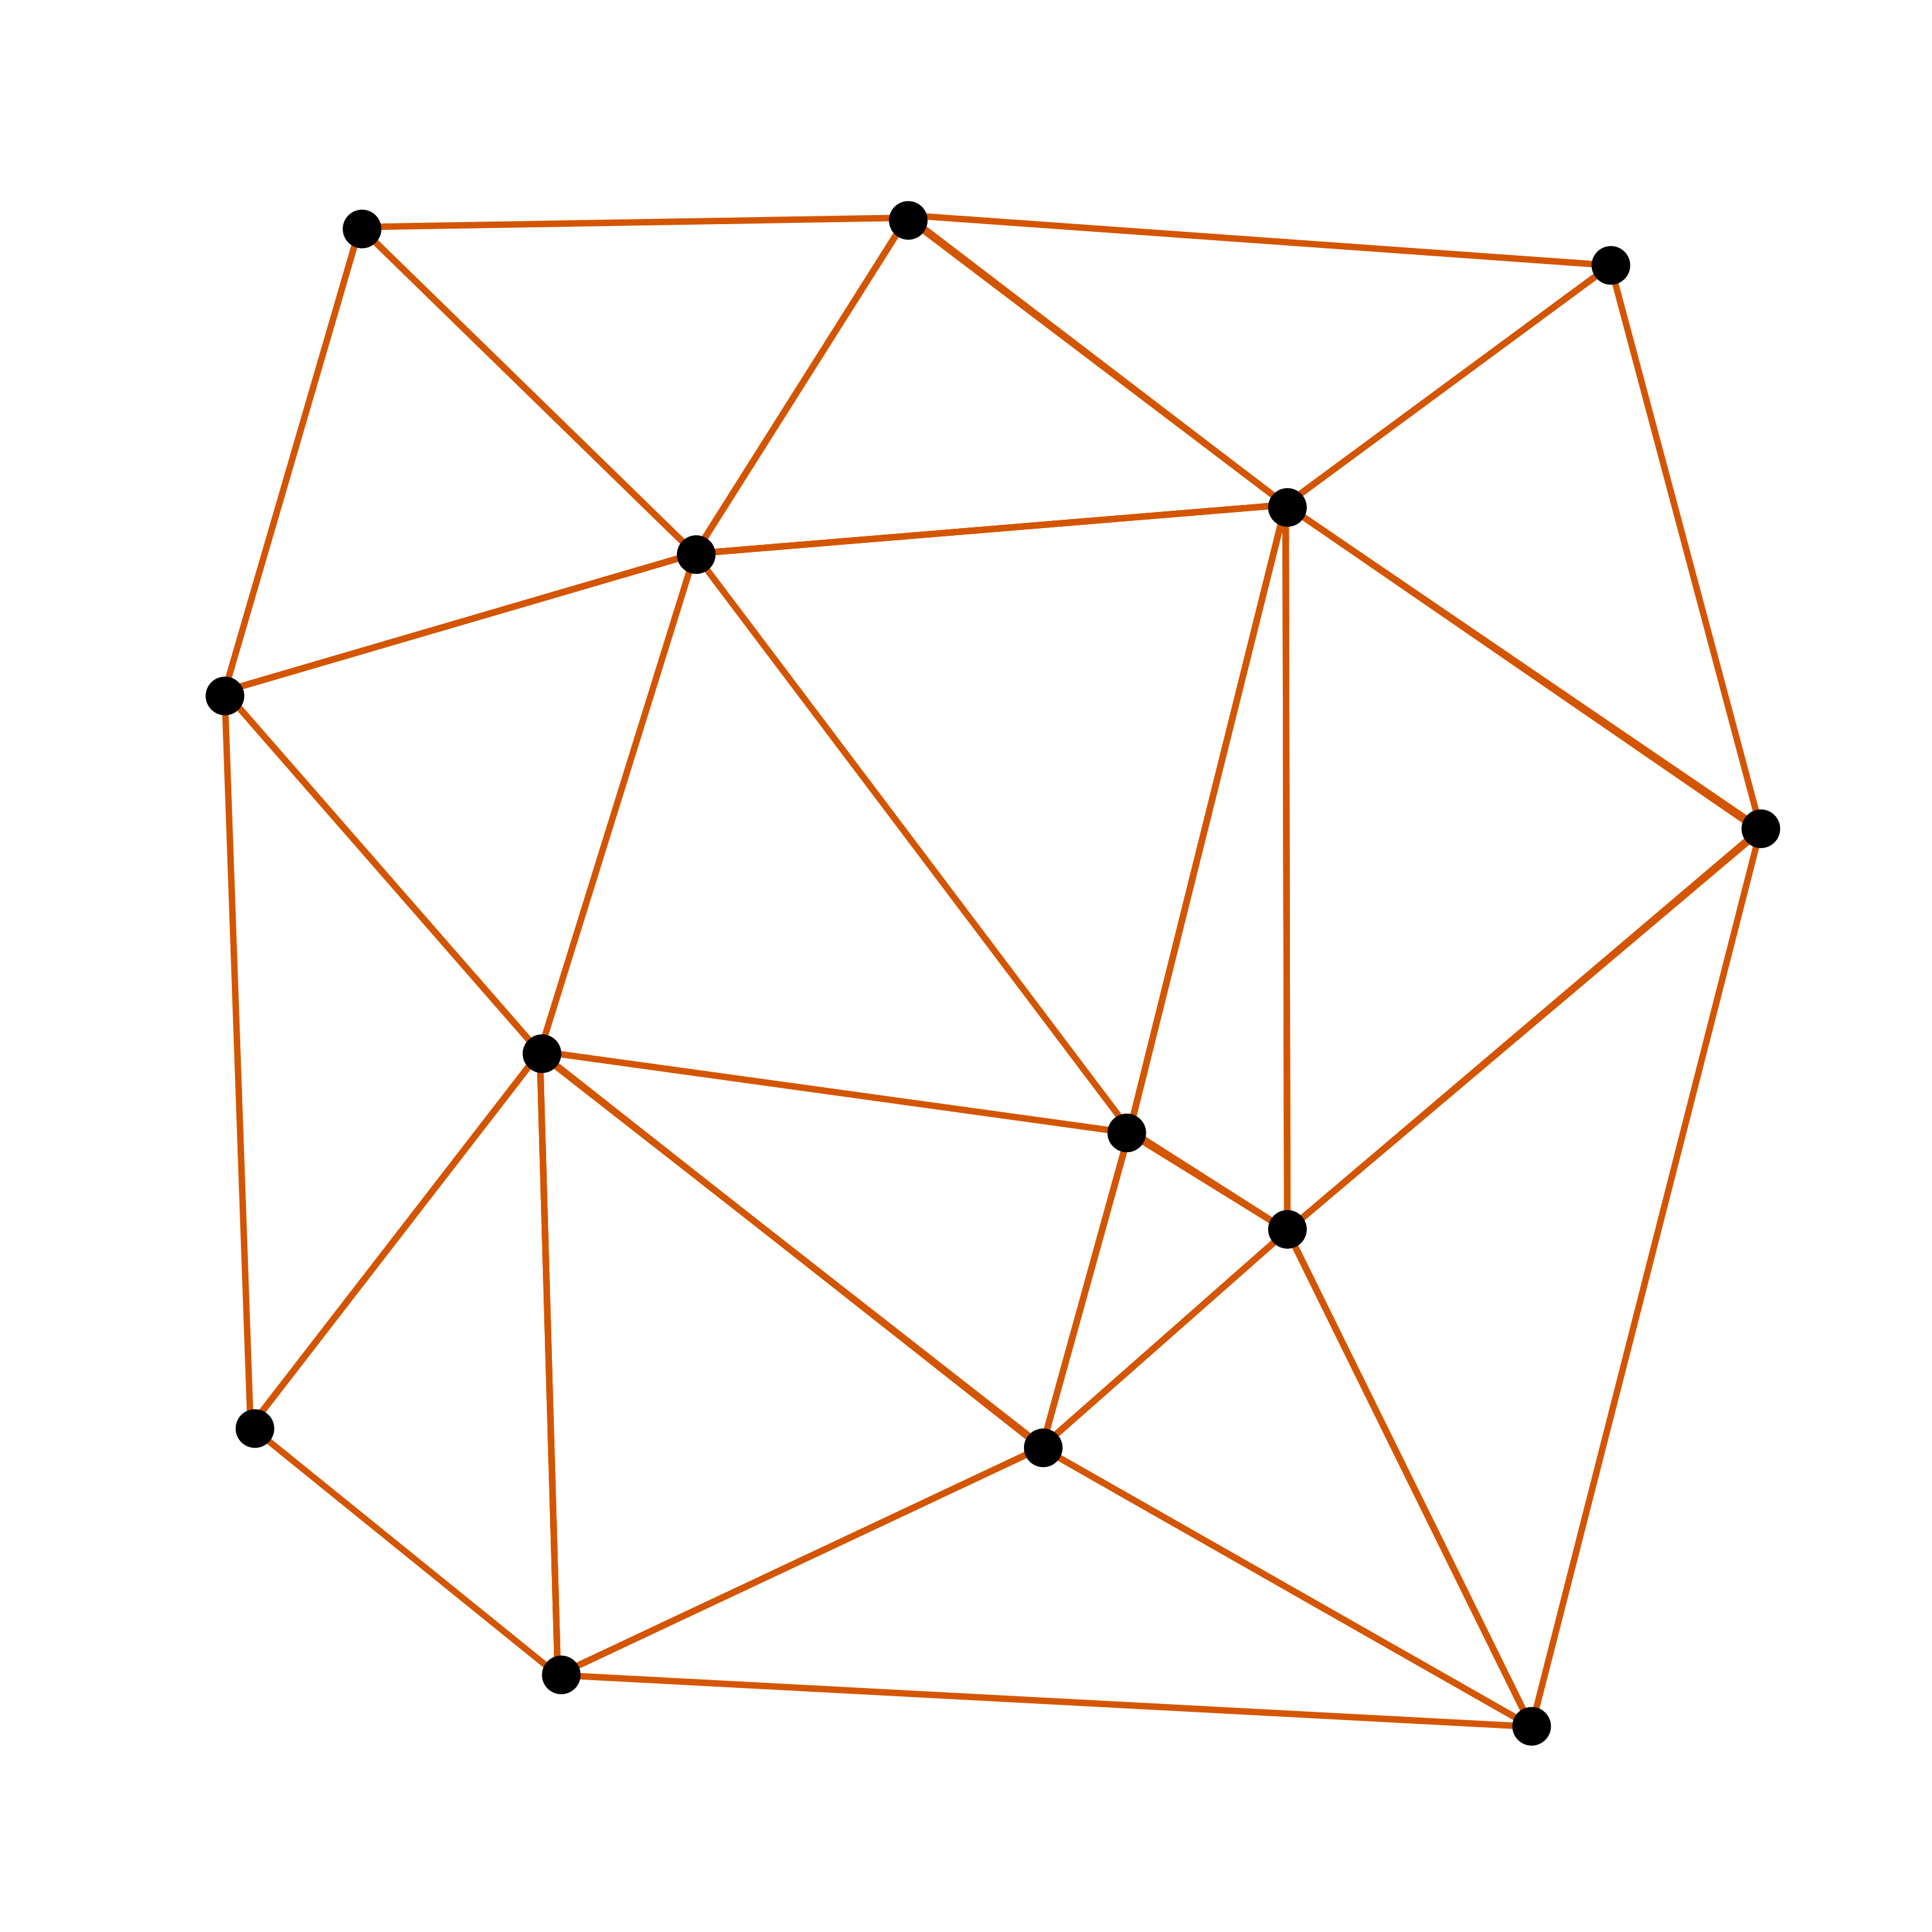
\includegraphics[width=0.3\textwidth]{pictures/Delaunay-Triangulation1.png}
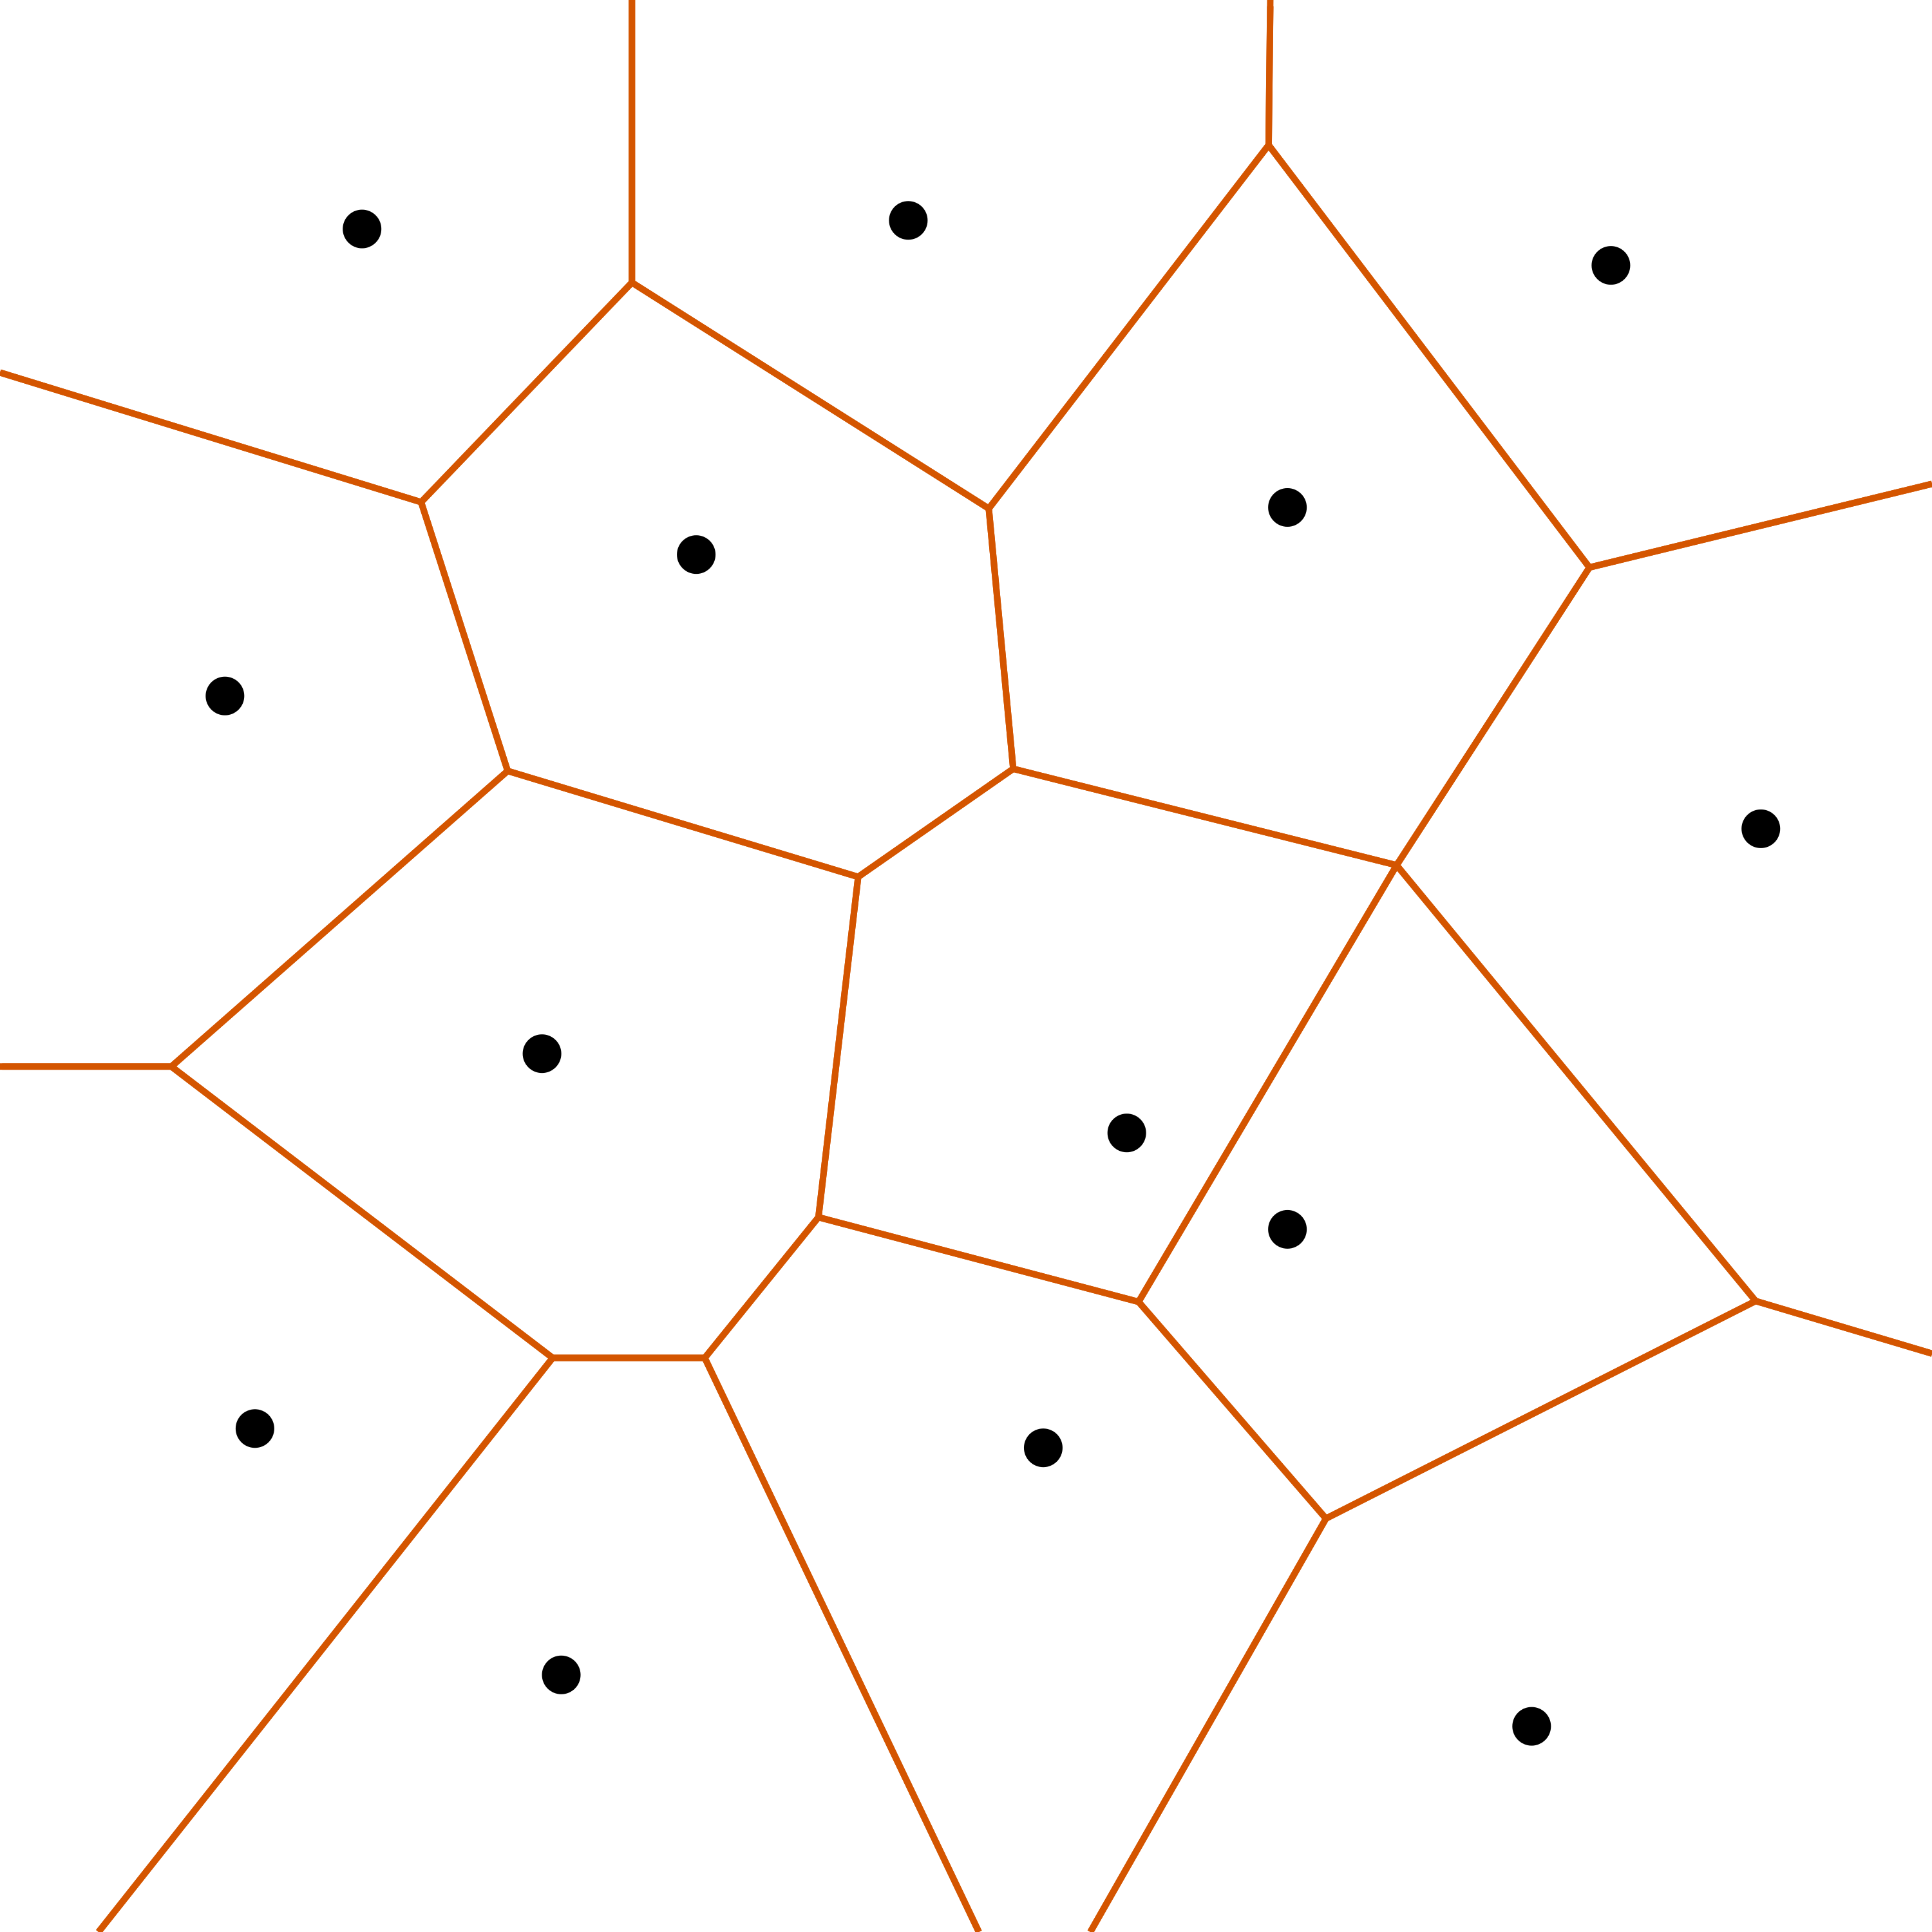
\includegraphics[width=0.3\textwidth]{pictures/Delaunay-Triangulation2.png}
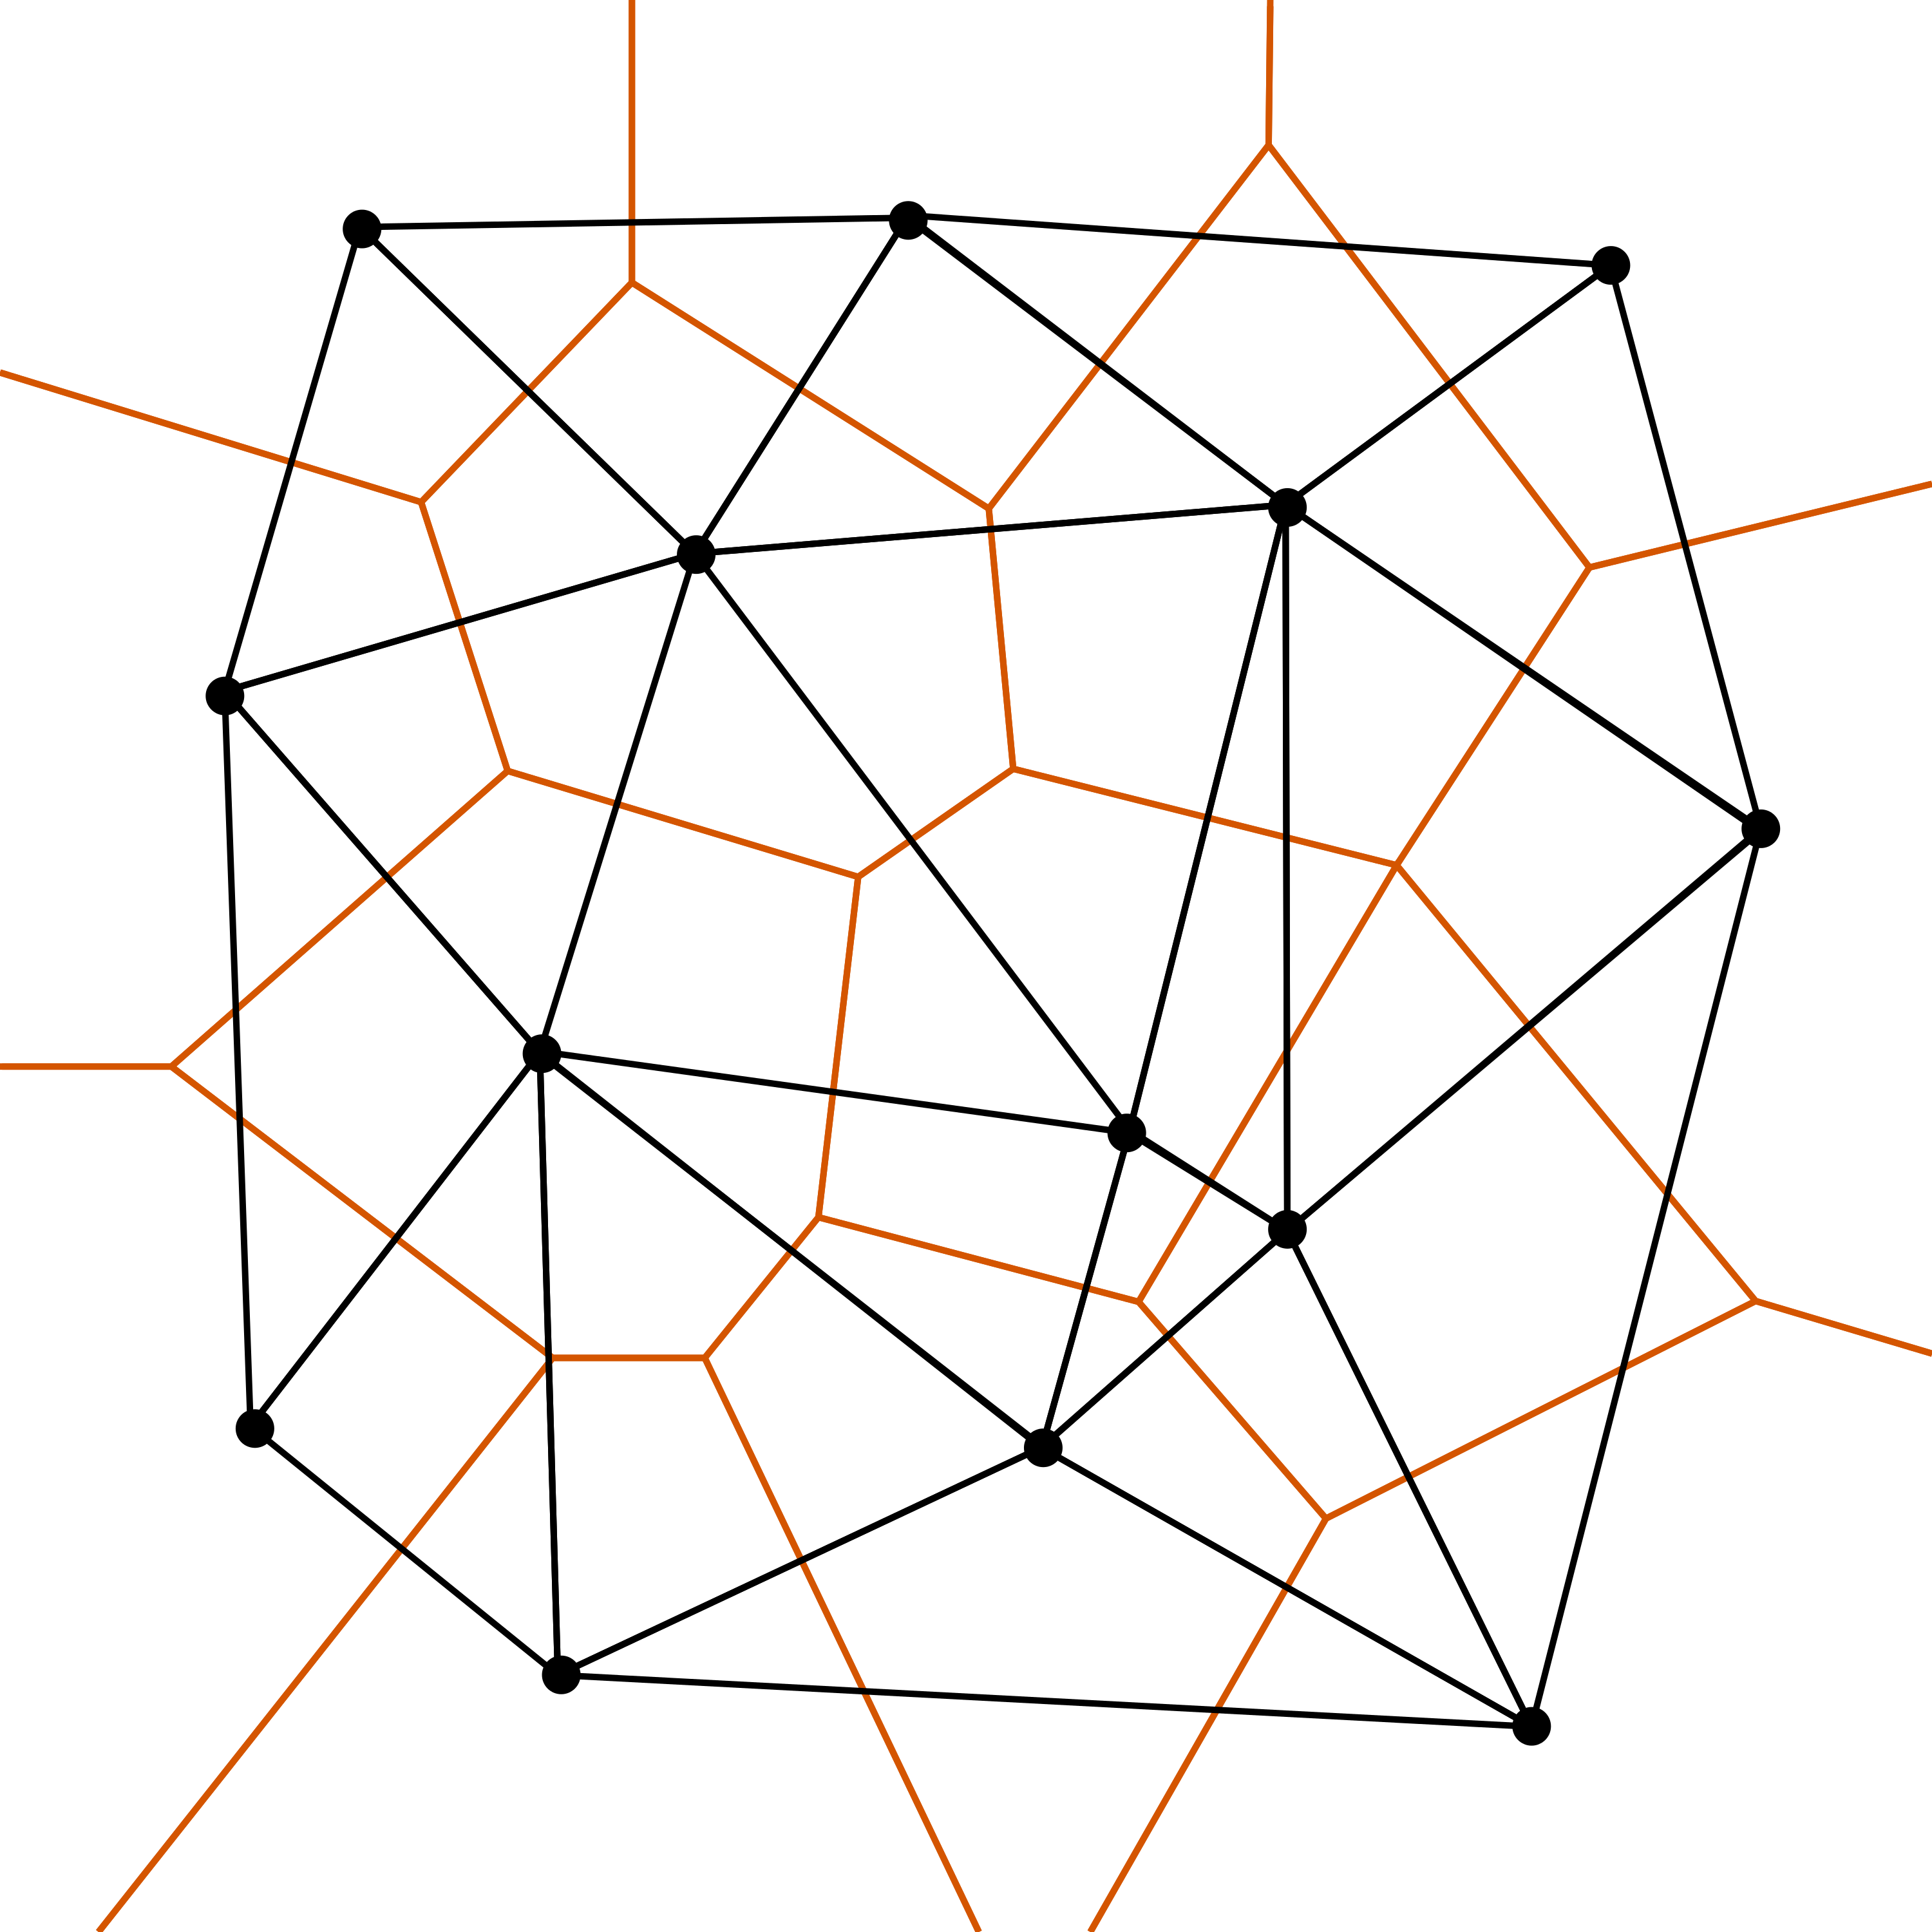
\includegraphics[width=0.3\textwidth]{pictures/Delaunay-Triangulation3.png}
 \caption[Close up of \textit{Hemidactylus} sp.]{
A triangulation of a set of points (left), the corresponding Voronoi diagram (middle) and the overlapping of the triangulation and the Voronoi diagram, emphasizing the dual relationship (right).}
\end{figure}

\subsection{Arrangement}
\label{sec:arrangement}
Given a set of planar curves, the arrangement is the subdivision of the plane into zero-dimensional, one-dimensional and two-dimensional cells, called vertices, edges and faces, respectively induced by the given curves. \hyperref[ref:cgal]{1}

\subsection{The Set Cover Problem}
Given a set $\mathcal A$ of sets of numbers, the set cover problem is the problem of finding a minimal subset $\mathcal B$ of $\mathcal A$, so that the union of the sets in $\mathcal B$ is equal to the union of all elements of $\mathcal A$.

\subsubsection{Example}
Let $\mathcal A$ =  \{\{1,2\}, \{2,3\}, \{2,5\}, \{3,5\}\}. The union of all sets of $\mathcal A$ is \{1,2,3,5\}. \newline
The subset $\mathcal B_1$ = \{\{1,2\}, \{2,3\}\} has the union \{1,2,3\} and does not cover the set $\mathcal A$. \newline
The subset $\mathcal B_2$ = \{\{1,2\}, \{2,3\}, \{2,5\}\} has the union \{1,2,3,5\} that covers $\mathcal A$, but it is not minimal. \newline
A minimal solution is $\mathcal B_3$ = \{\{1,2\}, \{3,5\}\}. \newline
The set cover problem is known to be NP-complete.\hyperref[ref:karp]{4}
\section{Problem formulation}
Given a set $\mathcal{R}$ of red points, find a set $\mathcal{B}$ of blue points such that in the Voronoi diagram of $\mathcal{R} \cup \mathcal{B}$, no two regions corresponding to points in $\mathcal{R}$ are incident to each other. For the Delaunay triangulation of $\mathcal{R} \cup \mathcal{B}$, this means that there is no edge connecting two red points. The conjecture that |$\mathcal{B}$| = |$\mathcal{R}$| is needed in an optimal solution is to be experimentally explored.


\section{Background}
\subsection{Upper and lower bounds}
Given a set $\mathcal{R}$ of red points with $N = |\mathcal{R}|$, it has been shown \hyperref[ref:blocking]{2} that at least N-1 points are needed to solve this problem. This is exemplified in the picture below, and always applies to the special case when all points lie in row. In the general case, it has been shown that for $N>2$ there are cases where at least N blue points are required to solve the problem.

\begin{figure}[hb]
\centering
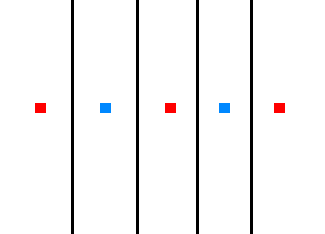
\includegraphics[width=0.3\textwidth]{pictures/N-1solution.png}
 \caption[Close up of \textit{Hemidactylus} sp.]
{Example of points not in general position, having a solution with N-1 blue points.}
\end{figure}

In the general case, it has been proved \hyperref[ref:blocking]{2} that at most $3N/2$ blue points are needed to solve the problem, and in the case where the points in  $\mathcal{R}$ are in convex position, $5N/2$ points are sufficient. It has been conjectured that $N$ points are sufficient to solve the problem in the general case.


\subsection{complexity}
Although not yet shown, the problem is suspected to be NP-hard \hyperref[ref:blocking]{2}, as a similar problem has been proven to be NP-hard. \hyperref[ref:alexander]{3}

\section{Algorithms}
\subsection{General outline}
\label{ref:Algorithm}
\begin{enumerate}
\item
For the set $\mathcal P$ of points (both red and blue) find the delaunay triangulation.
\item
\label{alg:part2}
For each edge connecting two red points in the triangulation, \hyperref[sec:findCircle]{find a circle} with the two points on its perimeter and add these to the (possibly empty) set of circles $\mathcal C$.
\item
Calculate the \hyperref[sec:arrangement]{arrangement} $\mathcal A$ of the circles $\mathcal C$.
\item
\hyperref[sec:findPoints]{Find a set of points} $\mathcal P^*$, so that for every face in the arrangement $\mathcal A$, exactly one point is located in the interior. For every point $\rho  \in \mathcal P^*$ and every circle $\varsigma$ in $\mathcal C$, determine whether $\rho$ is in the interior of $\varsigma$.
\item
\hyperref[sec:gurobi]{Find a minimum subset} of $\mathcal P^*$, so that every circle in $\mathcal C$ is covered by at least one point.
\item
Calculate a triangulation for the set of points $\mathcal P^* \cup Red(\mathcal P )$, where  $Red(\mathcal P )$ denotes the set of red points in $\mathcal P$.
\item
For every red edge still in the triangulation, calculate the length of its dual in the voronoi graph. If no red edges exists, terminate. If the length is sufficiently small, use \hyperref[sec:rand]{random search } to find an optimal solution. Otherwise, restart from \hyperref[alg:part2]{2}.
\end{enumerate}

\subsection{Finding circles corresponding to unsatisfied edges}
\label{sec:findCircle}
Following the terminology used by the CGAL-project, a {\bf line} is a line unbounded on both sides, whereas an line that is bounded on one side is called a {\bf ray} and when bounded on both sides it is called a {\bf segment}. The approach for choosing circles depends on which type of voronoi edge is to be blocked. Given a voronoi edge, corresponding to the neighbouring points $p_1$ and $p_2$, there are the following cases:

\begin{enumerate}
\item
For a {\bf line}, the smallest possible circle is chosen. This is the circle with its centre in the middle of $p_1$ and $p_2$, and a radius such that $p_1$ and $p_2$ are on its perimeter. A line only occurs in the voronoi diagram in the trivial case where all points lie in a straight line.
\item
Note that a {\bf ray} in the voronoi diagram is always associated with two points on the convex hull, for which infinitely large circles exist with the points $p_1$ and $p_2$ on its perimeter. In this case, a circle is randomly chosen.
\item
For a {\bf segment}, the circle with $p_1$ and $p_2$ on its perimeter, and its centre on the midpoint of the segment is chosen.
\end{enumerate}

\subsection{Finding a point in the interior of a face}
\label{sec:findPoints}
A relatively difficult task proved to be that of finding a point in the interior of an arbitrary face, given two point $p_1$ and $p_2$ known to be on the boundary of the face. The following algorithm was used.

\begin{figure}[hb]
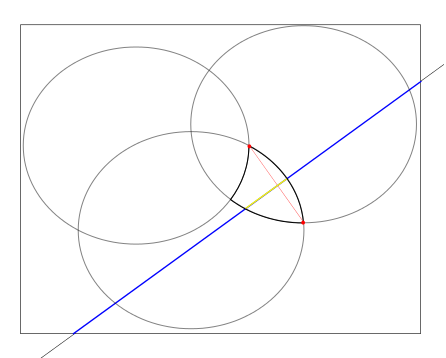
\includegraphics[width=0.4\textwidth]{pictures/PointInFace.png}
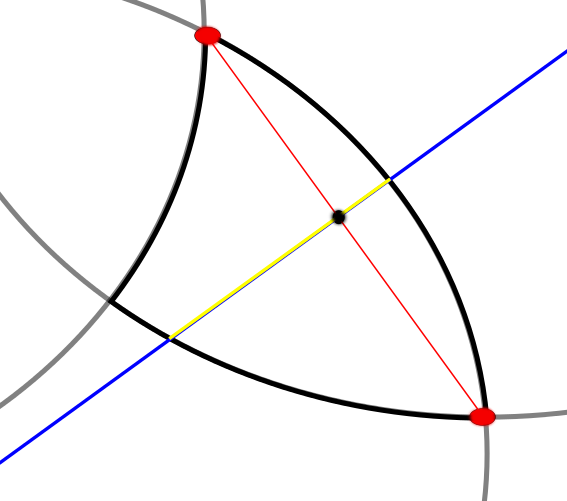
\includegraphics[width=0.3\textwidth]{pictures/PointInFace2.png}
 \caption[Close up of \textit{Hemidactylus} sp.]
   {ARE WE USING THIS SECTION AT ALL?.}
\end{figure}
\begin {itemize}
\item
Find the point $p_m$ in the middle of $p_1$ and $p_2$. If this point is inside the face, chose this point. (WE DON'T ACTUALLY DO THIS YET)
\item
Find the line $l$ going through $p_m$ and is perpendicular to the edge between $p_1$ and $p_2$.
\item
Find the segment $s$ that is the intersection of $l$ and the smallest rectangle large enough to contain all circles of the arrangement. This step is needed because a CGAL function needs an object of type segment as input. We describe this step here for the sake of completeness.
\item
Find the segment that is the intersection of the segment $s$ and the face itself.
\item
Any point except the endpoints of this segment are inside the face. The midpoint of the segment is chosen.
\end{itemize}

\subsection{Finding a minimal subset of points}
\label{sec:gurobi}
The problem of finding a minimal subset of a set of points $\mathcal P^*$, so that at least one point in $\mathcal P$ is in the interior of each circle in $\mathcal C$, is exactly that of the set covering problem. The problem is easily stated in terms of an integer programming problem, and can thus be solved relatively efficiently with an integer programming solver, such as Gurobi.
\subsubsection{Pseudo code }
For every point $\rho_i \in \mathcal P^*$, let $x(\rho_i)$ be a boolean, set to 1 if the point $\rho_i$ appears in a solution and 0 otherwise. Also, for every circle $\varsigma_j \in \mathcal C$, let $\varsigma_j (\rho_i)$ be 1 if point $\rho_i$ lies in the interior of $c_j$ and 0 otherwise.



\begin{lstlisting}[mathescape]
Minimize: $\sum\limits_{ \rho \in \mathcal P^*} x(\rho_{i}) \hspace{70pt} $
Constraint: $\sum\limits_{ \rho \in \mathcal P^*} \varsigma_j(\rho_i) \geq 1 \hspace{40pt}$ for each $\varsigma \in \mathcal C$
\end{lstlisting}

\subsection{Refining a near-optimum through random search}
\label{sec:rand}
Random search is a direct search method that does not require the derivative of the function to be minimized. It is algorithmically simple, and in general terms work as follows:

To minimize a function $f : \mathds{R}^n \rightarrow \mathds{R}$, start with a (potentially random)  solution $x :  \mathds{R}^n$. 

\begin{lstlisting}[mathescape]
while (f(x) > 0
	Generate a new candidate solution y, in the neighbourhood of x
	if f(y) < f(x)
		replace the current solution x with y.
\end{lstlisting}

There are several candidates for choosing the objective function \emph{f}, for example the number of red delaunay circles or red voronoi edges. For this problem, we have chosen the sum the squared lengths of all red voronoi edges.

\section{Results}

\subsection{Graphical interface}
In order to easily specify new problems, and to visualize the process of solving the problems, a minimalistic graphical interface is used. It has methods for adding, moving and removing points. It automatically updates and draws the voronoi diagram corresponding to the set of points, and also a set of delaunay circles corresponding to the red edges in the voronoi diagram.

Additionally, methods for saving and loading configurations were added to simplify testing and debugging.

\begin{figure}[h]
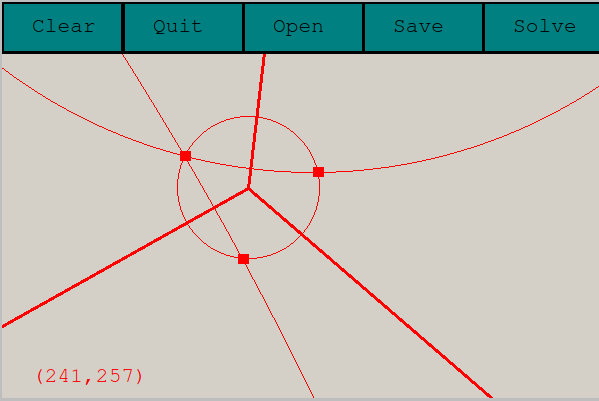
\includegraphics[width=0.4\textwidth]{pictures/gui.png}
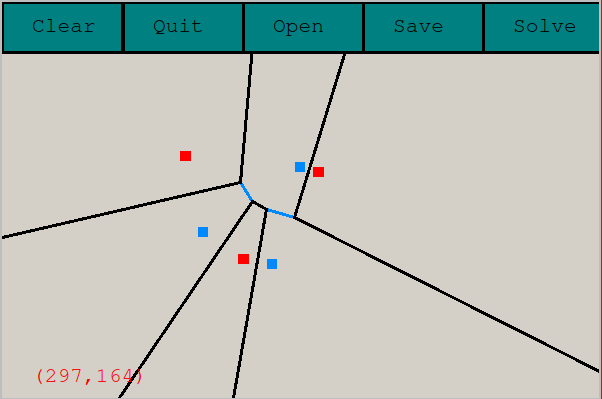
\includegraphics[width=0.4\textwidth]{pictures/guisolved.png}
 \caption[Close up of \textit{Hemidactylus} sp.]
   {An example of a problem configuration (left) and a found solution to the same problem (right).}
\end{figure}

\subsection{Speed}
The problem of finding a blocking set of blue points is computationally hard, since the set-cover problem is NP-hard and also by its own, assuming the conjuncture in \hyperref[ref:blocking]{2} is true. This complexity is reflected in the time it takes to solve a problem, shown in figure 4.

The figure shows the average time of solving a problem, with between 7 and 12 points. The program was run on forty randomely generated problems each (not the same forty). Due to the existence of local minima in the search space, there is a small risk that a run takes unusually long time. Such statistical \emph{outliers} greatly impact the total average, and thus both a graph with and without these outlier values have been included.

\begin{figure}[h]
\begin{center}
\label{ref:speed}
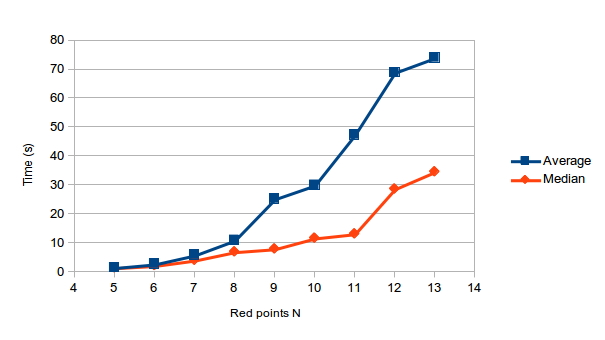
\includegraphics[width=0.8\textwidth]{pictures/speedStats.png}
 \caption[Close up of \textit{Hemidactylus} sp.]
   {Graph showing average time to find a solution, for problems of different size. The average is based on forty runs, and the results are shown both with and without outlier values.}
\end{center}
\end{figure}


In all the tested problems, the number of blue points in the final solution was the same as the number of red points in the original problem.


\subsection{Exact or Inexact Points}
A design issue was that of finding a point in every face of the arrangement (step 4 in section  \hyperref[ref:Algorithm]{4.1}). The algorithm presented in section \hyperref[sec:findPoints]{4.3} provides satisfying results, but is high on computation.

An alternative approach is to simply chose two points on the boundary of a face, and chose the middle point. Such a point will be within the face 50\% of the cases, since the boundary of the face in a restricted area is convex or concave with the same probability. 

This latter approach is computationally easy, but does not fully fulfill the requirement of the algorithm. If is not known if this fact leads to undesired behavior in some cases, for example non-optimal solutions or non-convergence. The gain in time, compared to the secure algorithm in 4.3, is shown in the graph below.



\section{Conclusions}
The purpose of this project has been to experimentally explore the claim, that in an optimal solution |$\mathcal{B}$| = |$\mathcal{R}$|. It must be noted that this can be falsified through experimentation by finding a counter-example to the claim, but it can never be experimentally proven. During testing, no counter-examples to the claim have been found, leaving us to believe that this conjecture is in fact true.

\section{Discussion}
During the course of this project, we have used our tool to solve a large amount of problem, but with the big limitation with respect to performance. Due to the exponential complexity of this problem (shown in \hyperref[ref:speed] {figure 7}), we have been limited to problems of a relatively small size. To more fully investigate this claim, the solver would likely need to be improved.

One way to do this is to more fully investigate how and when random search is effective. During our testing, a random search stage was entered when the total length of the red segments in the voronoi diagram was smaller than 300*N. This is a very course estimation, which if too large inevitably leads to a local minima, and if to small means the problem solved faster. It is also likely that using a similar but more sophisticated technique, such as tabu search, would be more effective.


\begin{itemize}
\item
Random search has a few things to note. Local minima is always a problem. Then two things that can be optimized, but we don't have time; first the threshhold, where we decide to start doing an RA, second the amount of randomization used. Tabu search would probably work awesome.
\item
Complexity of our algorithm? 
\end{itemize}

\section{Tools}
In this project, a set of tools and libraries were used. Most notably, the Computational Geometry Algorithms Library (CGAL) provides a vast number of efficient algorithms for different areas within computational geometry. In this project, we have had extensive use of the methods for calculating voronoi diagrams, triangulations and arrangements.

The Gurobi optimzer was used for solving the integer programming problem. It provides an easy-to-use C++-API.

We used git for revision control and to simplify our collaboration. The source code for the project is available at \url{https://github.com/martin-mfg/voronoi-thesis-tester}

\section{references}
\small
\begin{enumerate}
\item
\label{ref:cgal}
Ron Wein, Efi Fogel, Baruch Zukerman, and Dan Halperin

CGAL manual chapter 20, 2D Arrangements

http://www.cgal.org/Manual/3.3/doc\_html/cgal\_manual/Arrangement\_2/Chapter\_main.html

\item
\label{ref:blocking}
O. Aichholzer, R. Fabila-Monroy, T. Hackl, M. van Kreveld, A. Pilz, P. Ramos, und B. Vogtenhuber

Blocking Delaunay Triangulations. 

Proc. Canadian Conference on Computational Geometry, CCCG 2010, Winnipeg, August 9/11, 2010. 


% NP-hardness of a similar problem
\item
\label{ref:alexander}
M. de Berg, D. Gerrits, A. Khosravi, I. Rutter, C. Tsirogiannis and A. Wolff.

How Alexander the Great Brought the Greeks Together while Inflicting Minimal Damage to the Barbarians.

Proc. 26th European Workshop on Computational Geometry, pages 73-76, 2010.

\item
\label{ref:karp}
Richard M. Karp
Reducibility Among Combinatorial Problems.
In: R. E. Miller, J. W. Thatcher (Hrsg.): Complexity of Computer Computations. Plenum Press, New York 1972, S. 85-103.

\end{enumerate}


\subsection{images}
\begin{itemize}
\item
Delaunay circumcircles, GNU Free Documenation Licence, N\"u es

http://commons.wikimedia.org/wiki/File:Delaunay\_circumcircles.png

\item
Delaunay triangulation picture 1-3, public domain, user Capheiden 

http://upload.wikimedia.org/wikipedia/de/1/17/Voronoi-Delaunay.svg

http://upload.wikimedia.org/wikipedia/de/4/48/Voronoi-Diagramm.svg

http://upload.wikimedia.org/wikipedia/commons/1/1f/Delaunay-Triangulation.svg

\end{itemize}
\end{document}

